\section{Annexes}

\subsection{Annexe 1 : Preuve du théorème du biais de filiation relative par la variance}
\label{sec:Annexe 1}

Pour déterminer quel modèle influence le plus la structure finale du graphe $X$, nous évaluons la probabilité qu'un lien observé dans $X$ soit également présent dans un tirage indépendant de même espérance issu de l'un des modèles parents.

Soit $X$ le graphe issu du mélange $P_S = \alpha P_1 + (1-\alpha) P_2$. 
Soit $X^{(i)}$ un graphe témoin généré uniquement par le modèle $M_i$ via la probabilité $P_i$.
On cherche à comparer les probabilités de filiation $\mathcal{F}_i = P(X^{(i)} = 1 \mid X = 1)$.

\begin{description}
    \item[Hypothèse d'Équité :] $\mathbb{E}[P_1] = \mathbb{E}[P_2] = \rho$. Donc $\mathbb{E}[P_S] = \rho$.
    \item[Hypothèse d'Indépendance :] $\mathbb{E}[P_1 P_2] = \mathbb{E}[P_1]\mathbb{E}[P_2] = \rho^2$.
\end{description}

\subsection*{Probabilité de coïncidence conditionnelle d'un lien entre les tirages $X$ et $X^{(i)}$}

Par le théorème de Bayes, la probabilité qu'un lien du graphe final soit "partagé" avec celui issu du modèle témoin $M_i$ est :
\begin{equation}
    P(X^{(i)} = 1 \mid X = 1) = \frac{P(X = 1 \mid X^{(i)} = 1) \cdot P(X^{(i)} = 1)}{P(X = 1)}
\end{equation}

Sachant que $P(X = 1) = \mathbb{E}[P_S] = \rho$ et $P(X^{(i)} = 1) = \mathbb{E}[P_i] = \rho$, l'expression se simplifie en :
\begin{equation}
     P(X^{(i)} = 1 \mid X = 1) = P(X = 1 \mid X^{(i)} = 1) = \frac{P(X = 1 \cap X^{(i)} = 1)}{P(X^{(i)} = 1)}
\end{equation}

\subsection*{Calcul par l'espérance associée}

Le numérateur représente l'espérance du produit des variables de Bernoulli $X$ et $X^{(1)}$. Conditionnellement aux probabilités $P_1$ et $P_2$, ces tirages sont indépendants :

\begin{align}
    P(X = 1 \cap X^{(1)} = 1) &= \mathbb{E}[ \mathbb{E}[X \cdot X^{(1)} \mid P_1, P_2] ] \nonumber \\
    &= \mathbb{E}[ P_S \cdot P_1 ] \nonumber \\
    &= \mathbb{E}[ (\alpha P_1 + (1-\alpha) P_2) P_1 ] \nonumber \\
    &= \alpha \mathbb{E}[P_1^2] + (1-\alpha) \mathbb{E}[P_1 P_2]
\end{align}

En utilisant la relation $\mathbb{E}[P_1^2] = \text{Var}(P_1) + \rho^2$ et l'hypothèse d'indépendance $\mathbb{E}[P_1 P_2] = \rho^2$ :
\begin{align}
    P(X = 1 \cap X^{(1)} = 1) &= \alpha (\text{Var}(P_1) + \rho^2) + (1-\alpha) \rho^2 \nonumber \\
    &= \alpha \text{Var}(P_1) + \rho^2
\end{align}

\subsection*{Résultat : Ratio de filiation relative}

La probabilité de filiation pour chaque modèle, définie comme la probabilité qu'un lien du mélange soit également présent dans un tirage de même taille issu modèle parent, est donc donnée par :
\begin{equation}
    \mathcal{F}_1 = \frac{\alpha \text{Var}(P_1) + \rho^2}{\rho} \quad \text{et} \quad \mathcal{F}_2 = \frac{(1-\alpha) \text{Var}(P_2) + \rho^2}{\rho}
\end{equation}

Enfin, le ratio de filiation $\mathcal{R}_F = \frac{\mathcal{F}_1}{\mathcal{F}_2}$ donne :
\begin{equation}
    \mathcal{R}_F = \frac{\mathcal{F}_1}{\mathcal{F}_2}  = \frac{\alpha \text{Var}(P_1) + \rho^2}{(1-\alpha) \text{Var}(P_2) + \rho^2} \underset{\rho \ll 1}{\approx} \frac{\alpha \text{Var}(P_1)}{(1-\alpha) \text{Var}(P_2)}
\end{equation}

\newpage

\subsection{Annexe 2 : Liste des métriques et algorithmes de l'état de l'art utilisés regroupés par paradigme}
\label{sec:Annexe2}

Cette annexe liste de manière exhaustive les $22$ descripteurs structurels, nodaux et dyadiques extraits du graphe pour alimenter le méta-classificateur \textit{XGBoost}. Pour chaque métrique, $u$ et $v$ désignent la paire de sommets évaluée, et $\Gamma(u)$ représente le voisinage direct du nœud $u$.

\subsubsection{Le paradigme topologique}

Les caractéristiques nodales ($c_u$) entrent dans le modèle sous forme de paires $(c_u, c_v)$, tandis que les métriques de voisinage ou de chemin décrivent directement la dyade $(u, v)$.

\begin{table}[h]
\centering
\caption{Métriques topologiques nodales et dyadiques}
\label{tab:metriques_topo}
\begin{tabular}{lll}
\hline
\textbf{Acronyme} & \textbf{Nom complet} & \textbf{Formulation mathématique / Définition} \\
\hline
\texttt{degree} & Degré nodal & $k_u = |\Gamma(u)|$ \\
\texttt{pr} & PageRank & Probabilité stationnaire d'une marche aléatoire \\
\texttt{ppr} & PageRank Personnalisé & Vecteur stationnaire avec redémarrage forcé sur $u$ \\
\texttt{lcc} & Coeff. de Clustering Local & $C_u = \frac{2 |\{ (w,z) \in E \,:\, w,z \in \Gamma(u) \}|\} }{k_u(k_u-1)}$ \\
\texttt{and} & Degré Moyen des Voisins & $\frac{1}{k_u} \sum_{w \in \Gamma(u)} k_w$ \\
\texttt{dc} & Centralité de Degré & $k_u / (|V|-1)$ \\
\texttt{katz} & Centralité de Katz & $c_{\text{Katz}}(u) = \sum_{m=1}^{\infty} \beta^m (A^m)_{u}$ \\
\texttt{cn} & Voisins Communs & $|\Gamma(u) \cap \Gamma(v)|$ \\
\texttt{aa} & Index Adamic/Adar & $\sum_{w \in \Gamma(u) \cap \Gamma(v)} \frac{1}{\log k_w}$ \\
\texttt{ra} & \textit{Resource Allocation} & $\sum_{w \in \Gamma(u) \cap \Gamma(v)} \frac{1}{k_w}$ \\
\texttt{jc} & Coefficient de Jaccard & $|\Gamma(u) \cap \Gamma(v)| \,/\, |\Gamma(u) \cup \Gamma(v)|$ \\
\texttt{pa} & Attachement Préférentiel & $k_u \cdot k_v$ \\
\texttt{sp} & Plus Court Chemin & $\min(\text{longueur}(u \rightsquigarrow v))$, ou $42$ si disjoints \\
\hline
\end{tabular}
\end{table}

\subsubsection{Le paradigme des algorithmes de communautés}

Pour chaque algorithme, la caractéristique dyadique injectée est une valeur continue correspondant à la densité de liens observée entre les deux communautés auxquelles appartiennent respectivement les nœuds $u$ et $v$.

\begin{table}[h]
\centering
\caption{Algorithmes de détection de structures communautaires}
\label{tab:metriques_commu}
\begin{tabular}{lll}
\hline
\textbf{Acronyme} & \textbf{Nom complet} & \textbf{Fonction objectif / Modèle nul} \\
\hline
\texttt{louvain} & Algorithme de Louvain & Maximisation gloutonne de la modularité classique \\
\texttt{infomap} & Infomap & Minimisation du flux d'information (codage de Huffman) \\
\texttt{sbm} & \textit{Stochastic Block Model} & Maximum de vraisemblance sur blocs de Bernoulli \\
\texttt{leiden} & Algorithme de Leiden & Maximisation de modularité avec garantie de connexité \\
\texttt{surprise} & Évaluation par la \textit{Surprise} & Modèle nul hypergéométrique (densité de liens) \\
\texttt{significance} & \textit{Significance} & Modèle nul binomial (significativité statistique) \\
\hline
\end{tabular}
\end{table}

\subsubsection{Le paradigme des plongements géométriques (\textit{Embeddings})}

Les coordonnées de l'espace latent appris par parcours de graphe sont utilisées pour calculer une mesure de proximité vectorielle (distance euclidienne $\|\mathbf{z}_u - \mathbf{z}_v\|$)

\begin{table}[h]
\centering
\caption{Algorithmes d'apprentissage de représentations géométriques latentes}
\label{tab:metriques_embed}
\begin{tabular}{lll}
\hline
\textbf{Acronyme} & \textbf{Nom complet} & \textbf{Stratégie d'exploration de l'espace} \\
\hline
\texttt{deepwalk} & DeepWalk & Marches aléatoires uniformes + architecture \textit{Skip-gram} \\
\texttt{n2v\_homophily} & node2vec (Homophilie) & Marches biaisées au second ordre de type DFS ($p>1, q<1$) \\
\texttt{crosswalk} & CrossWalk & Marches biaisées aux frontières pour la \textit{fairness} \\
\hline
\end{tabular}
\end{table}


\subsection{Annexe 3 : Heatmap de la contribution de l'ensemble des métriques significativement utilisées par le modèle \textit{XGBoost} (top 20), moyenne sur 10 itérations}
\label{sec:Annexe3}


\begin{figure}
\includegraphics[width=\textwidth]{Plots/202 SHAPvals_top20_heatmap_sbmv4.png}
\caption{Evolution de l'importance du top 20 métriques, mesurée à travers la valeur absolue moyenne de leurs SHAP valeurs sur le dataset d'évluation (sur 10 itérations).} \label{fig4}
\end{figure}


\subsection{Annexe 4 : Evolution du coefficient de spearman entre les features et la \textit{Ground Truth} communautaire (à droite), et la \textit{Ground Truth} géométrique (à gauche) en fonction de $\alpha$ (moyenne sur 10 itérations).}
\label{sec:Annexe4}


\begin{figure}
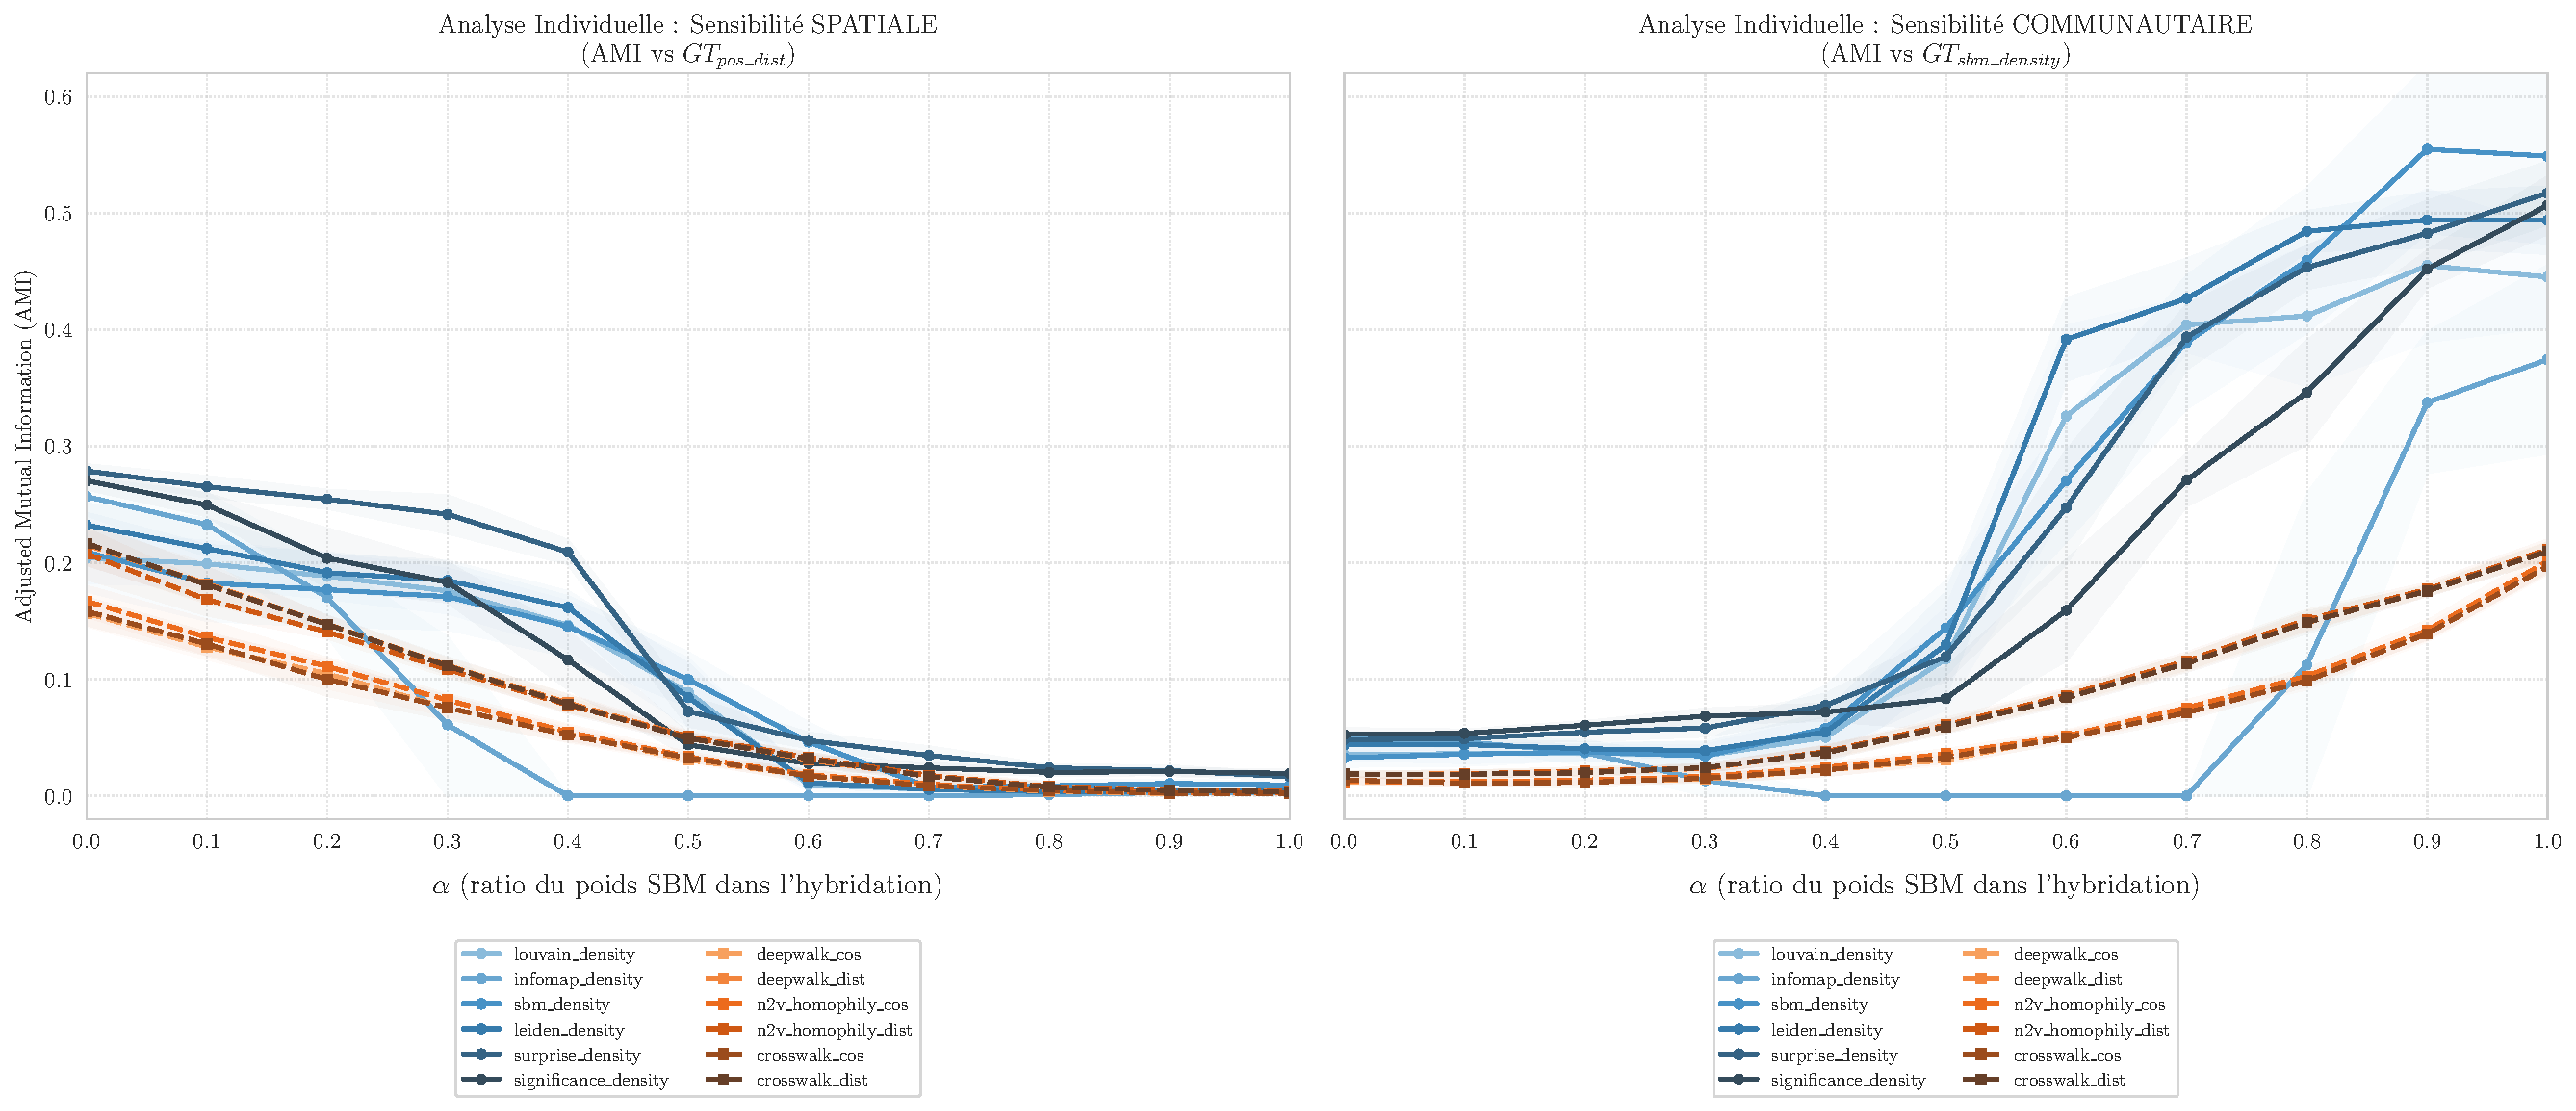
\includegraphics[width=\textwidth]{Plots/205 00_AMI_individual_features_VS_GT_comparison.pdf}
\caption{Evolution de l'Information Mutuelle Ajustée (AMI) entre les features et la \textit{Ground Truth} communautaire (à droite), et la \textit{Ground Truth} géométrique (à gauche) en fonction de $\alpha$ (moyenne sur 10 itérations).} \label{fig4}
\end{figure}


\subsection{Annexe 69 : Tables et graphes alternatifs mis de côté au cas où : }

\subsubsection{Table alternative à graph 1 SHAPvals GT\_pos et GT\_sbm pour validation}

\begin{table}[!ht]
\centering
\caption{Évolution des contributions SHAP globales moyennes de la \textit{Ground Truth} en fonction du ratio d'hybridation $\alpha$ (sur 10 expérimentations)}
\label{tab:validation_gt_shap}
\begin{tabular}{ccc}
\hline
\textbf{Ratio SBM ($\alpha$)} & \textbf{Contribution $\Phi_{\text{GT\_pos}}$} & \textbf{Contribution $\Phi_{\text{GT\_sbm}}$} \\
\hline
0.0 & 2,1644 $\pm$ 0,1245 & 0,2317 $\pm$ 0,0206 \\
0.1 & 1,8726 $\pm$ 0,0900 & 0,4158 $\pm$ 0,0533 \\
0.2 & 1,5545 $\pm$ 0,0554 & 0,5908 $\pm$ 0,0587 \\
0.3 & 1,3979 $\pm$ 0,0637 & 0,7387 $\pm$ 0,0348 \\
0.4 & 1,1828 $\pm$ 0,0692 & 0,8812 $\pm$ 0,0493 \\
0.5 & 1,1123 $\pm$ 0,0846 & 1,0491 $\pm$ 0,0498 \\
0.6 & 0,9279 $\pm$ 0,0564 & 1,1443 $\pm$ 0,0700 \\
0.7 & 0,8374 $\pm$ 0,0492 & 1,3730 $\pm$ 0,0538 \\
0.8 & 0,6641 $\pm$ 0,0530 & 1,5164 $\pm$ 0,0708 \\
0.9 & 0,4696 $\pm$ 0,0311 & 1,7690 $\pm$ 0,0415 \\
1.0 & 0,3167 $\pm$ 0,0300 & 2,2268 $\pm$ 0,1050 \\
\hline
\end{tabular}
\end{table}